\documentclass{article}
\usepackage[utf8]{inputenc} % Permite el uso de caracteres del Español
\usepackage[T1]{fontenc}
\usepackage{hyperref}
\usepackage{graphicx}
\usepackage{wrapfig}
\usepackage{subcaption}

% set font encoding for PDFLaTeX, XeLaTeX, or LuaTeX
\usepackage{ifxetex,ifluatex}
\newif\ifxetexorluatex
\ifxetex
  \xetexorluatextrue
\else
  \ifluatex
    \xetexorluatextrue
  \else
    \xetexorluatexfalse
  \fi
\fi

\ifxetexorluatex
  \usepackage{fontspec}
\else
  \usepackage[T1]{fontenc}
  \usepackage[utf8]{inputenc}
  \usepackage{lmodern}
\fi

\usepackage{hyperref}

\title{Evalución 2: \\ El Atractor de Lorenz, ejemplo de Caos dinámico.}
\author{Melissa Matrecitos Avila}
\date{26 de Abril de 2018}

% Enable SageTeX to run SageMath code right inside this LaTeX file.
% http://mirrors.ctan.org/macros/latex/contrib/sagetex/sagetexpackage.pdf
% \usepackage{sagetex}

\begin{document}
\maketitle

\section{Introducción}

El sistema de Lorenz, que lleva su nombre gracias a Edward Lorenz, es un sistema de ecuaciones diferenciales ordinarias. Se caracteriza por tener soluciones caóticas para ciertos valores de parámetros y condiciones iniciales. Cuando estas soluciones se trazan, se asemejan a una mariposa o al ocho.

En 1963, Edward Lorenz desarrolló un modelo matemático simplificado para la convección atmosférica. El modelo es un sistema de tres ecuaciones diferenciales ordinarias conocidas ahora como las ecuaciones de Lorenz:

\centerline {$\displaystyle \frac{dx}{dt}=\sigma(y-x)$}
\centerline {$\displaystyle \frac{dy}{dt}=x(\rho-z)-y$}
\centerline {$\displaystyle \frac{dz}{dt}=xy-\beta z$}

Para la realización del examen se utilizó el sistema de Lorenz para hacer simulaciones de sistemas caóticos aplicando los conocimientos aprendidos sobre la solución de ecuaciones diferenciales, haciendo uso de las herramientas de Phyton.

\section{Resultados}
A continuación se muestran las gráficas obtenidas para distintos valores de las constantes $ \sigma, \rho  \textup{ y } \beta$, de este modo se puede resaltar la influencia que tienen estas en los sistemas caóticos. Además en el repositorio de Github se encuentran las animaciones de las soluciones.

\subsection{Ejemplo 1}
Valores: $\sigma = 10, \beta = 8/3 \textup{ y } \rho = 28$:
En la primera gráfica se muestra la fase en 3 dimensiones del atractor de Lorenz, donde claramente se observan dos puntos que son orbitados en distintas direcciones.
\begin{center}
    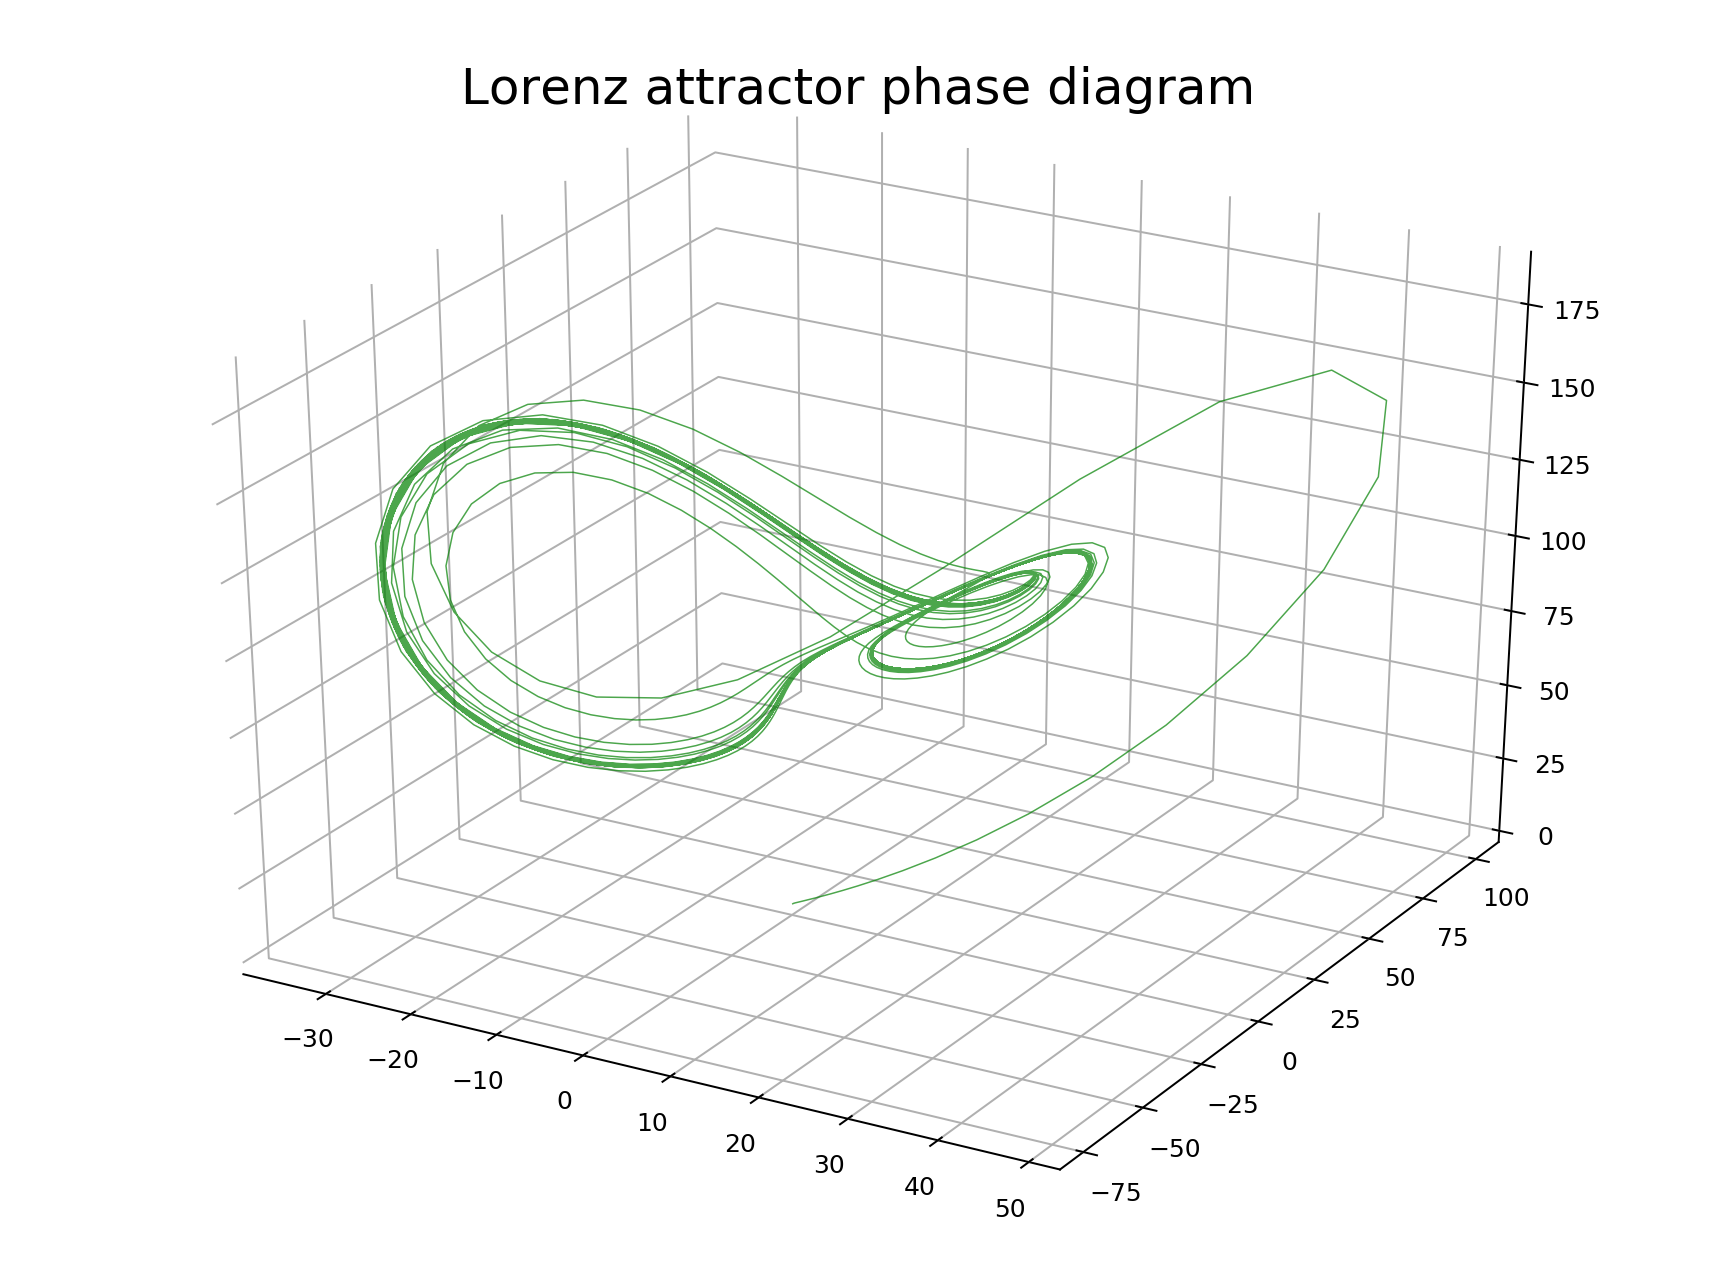
\includegraphics[width=1\textwidth]{lorenz-attractor-3d.png}
\end{center}
Las siguientes gráficas muestran distintas perspectivas de la gráfica anterior,es decir la proyección de la figura sobre distintos planos, en este caso son los planos xy, xz y yz respectivamente. 
\begin{center}
    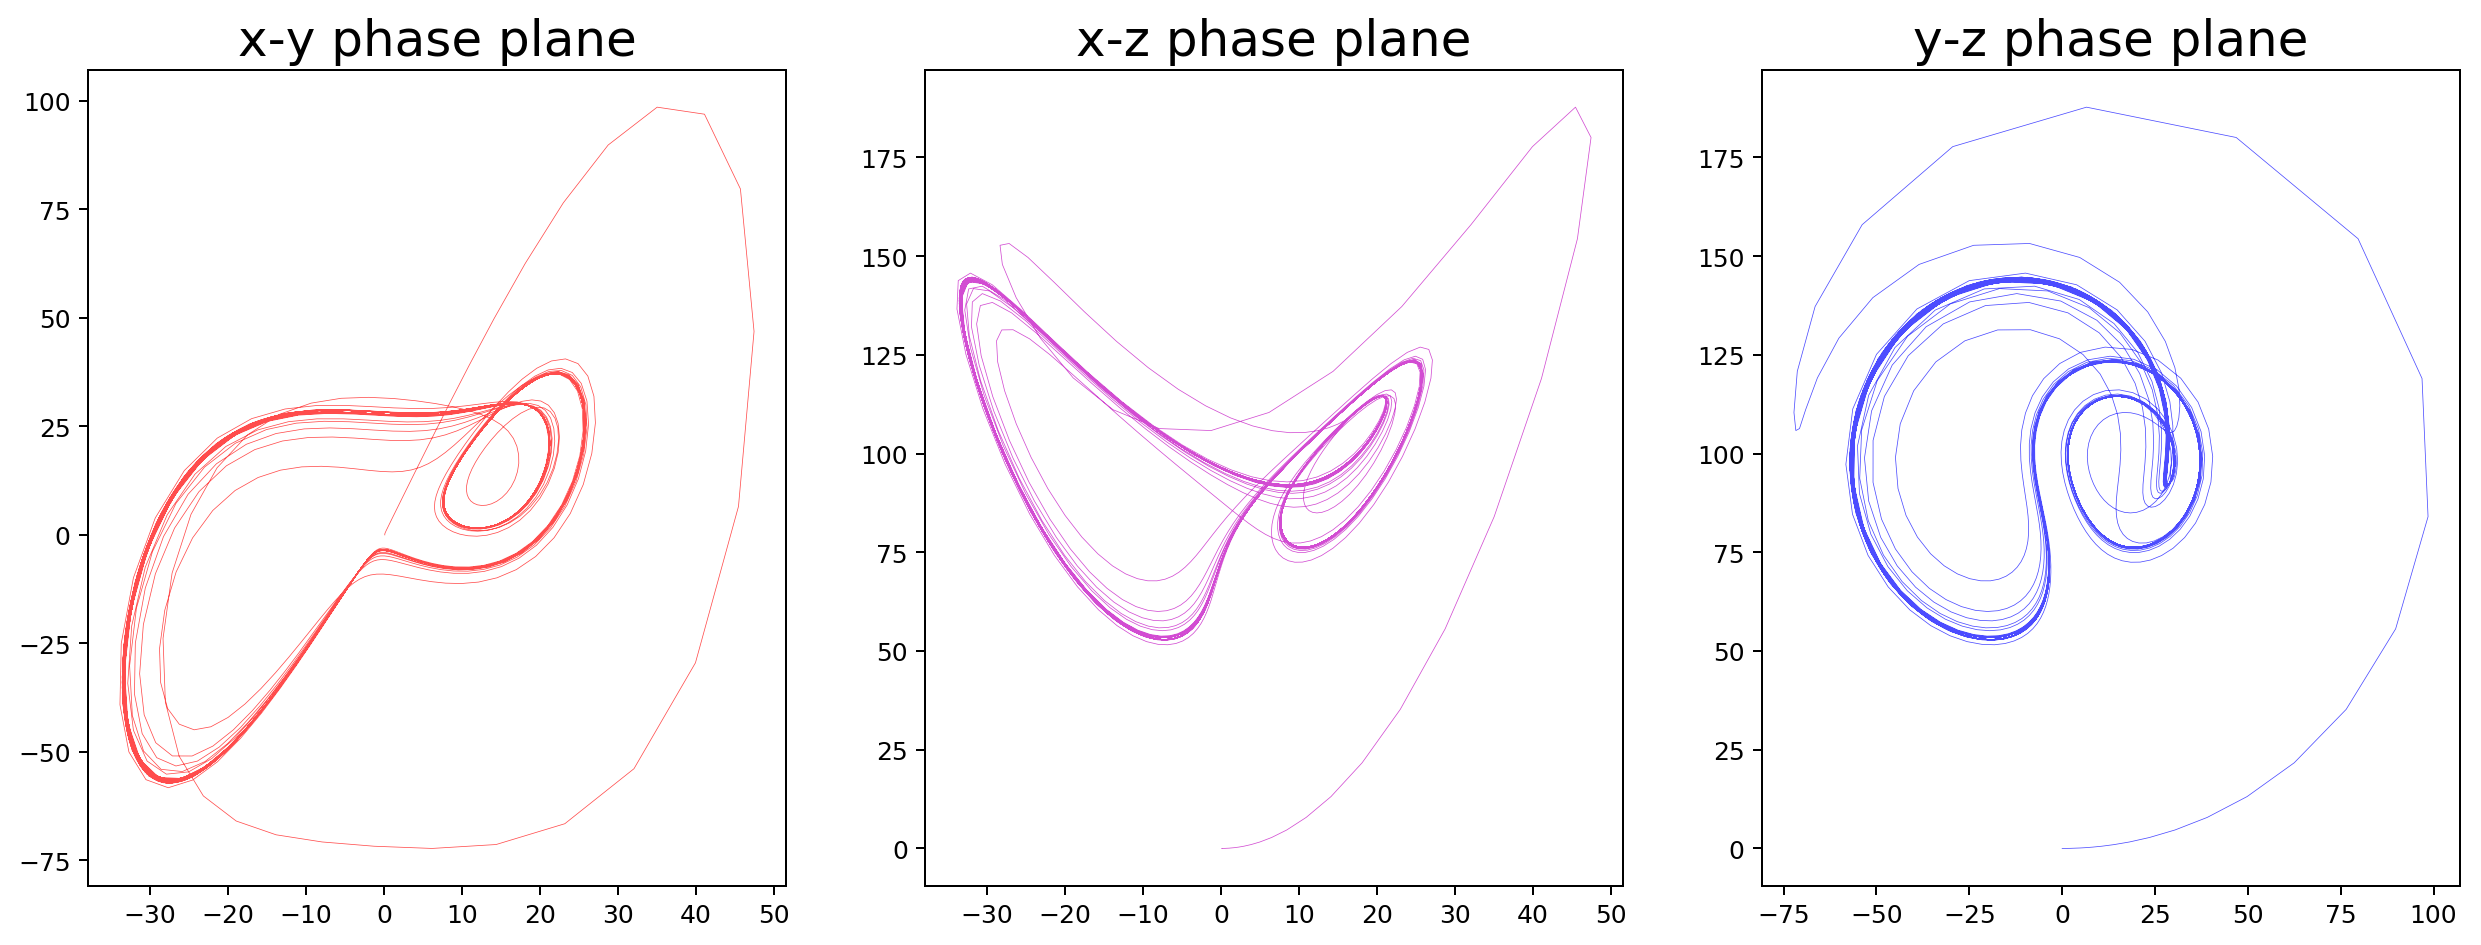
\includegraphics[width=1\textwidth]{lorenz-attractor-phase-plane.png}
\end{center}
A continuación se muestran las posiciones de x, y y z con respecto al tiempo, con el fin de comparar sus comportamientos. Se puede percibir como las variables x y y están casi sobre puestas, mientras que la variable z toma otros valores, sin embargo tienen un movimiento muy parecido.
\begin{center}
    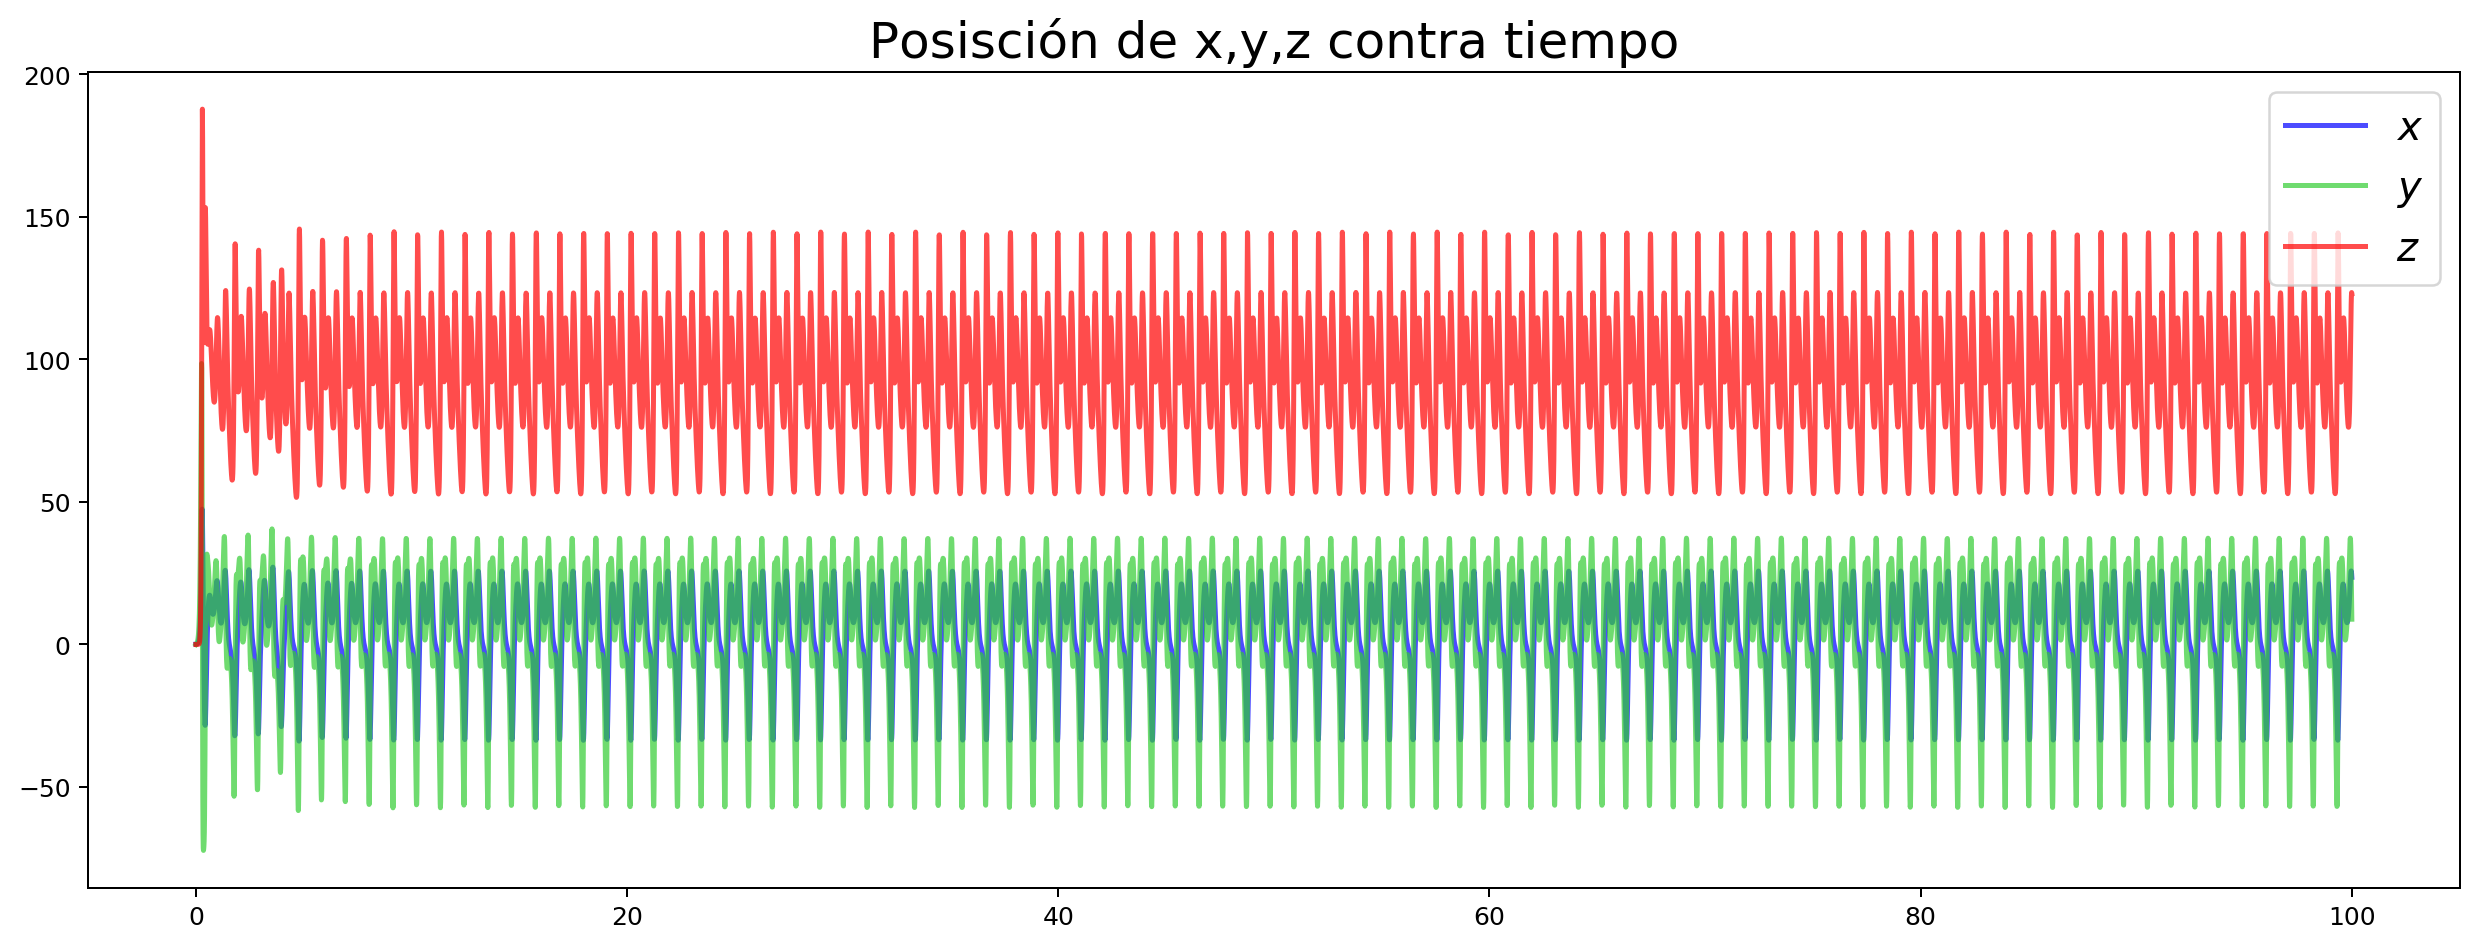
\includegraphics[width=1\textwidth]{Posicion.png}
\end{center}
Por último, se muestra un "zoom" a la gráfica anterior,tomando un intervalo de tiempo de 50 a 60 segundos, permitiendo observar mejor el comportamiento de las variables.
\begin{center}
    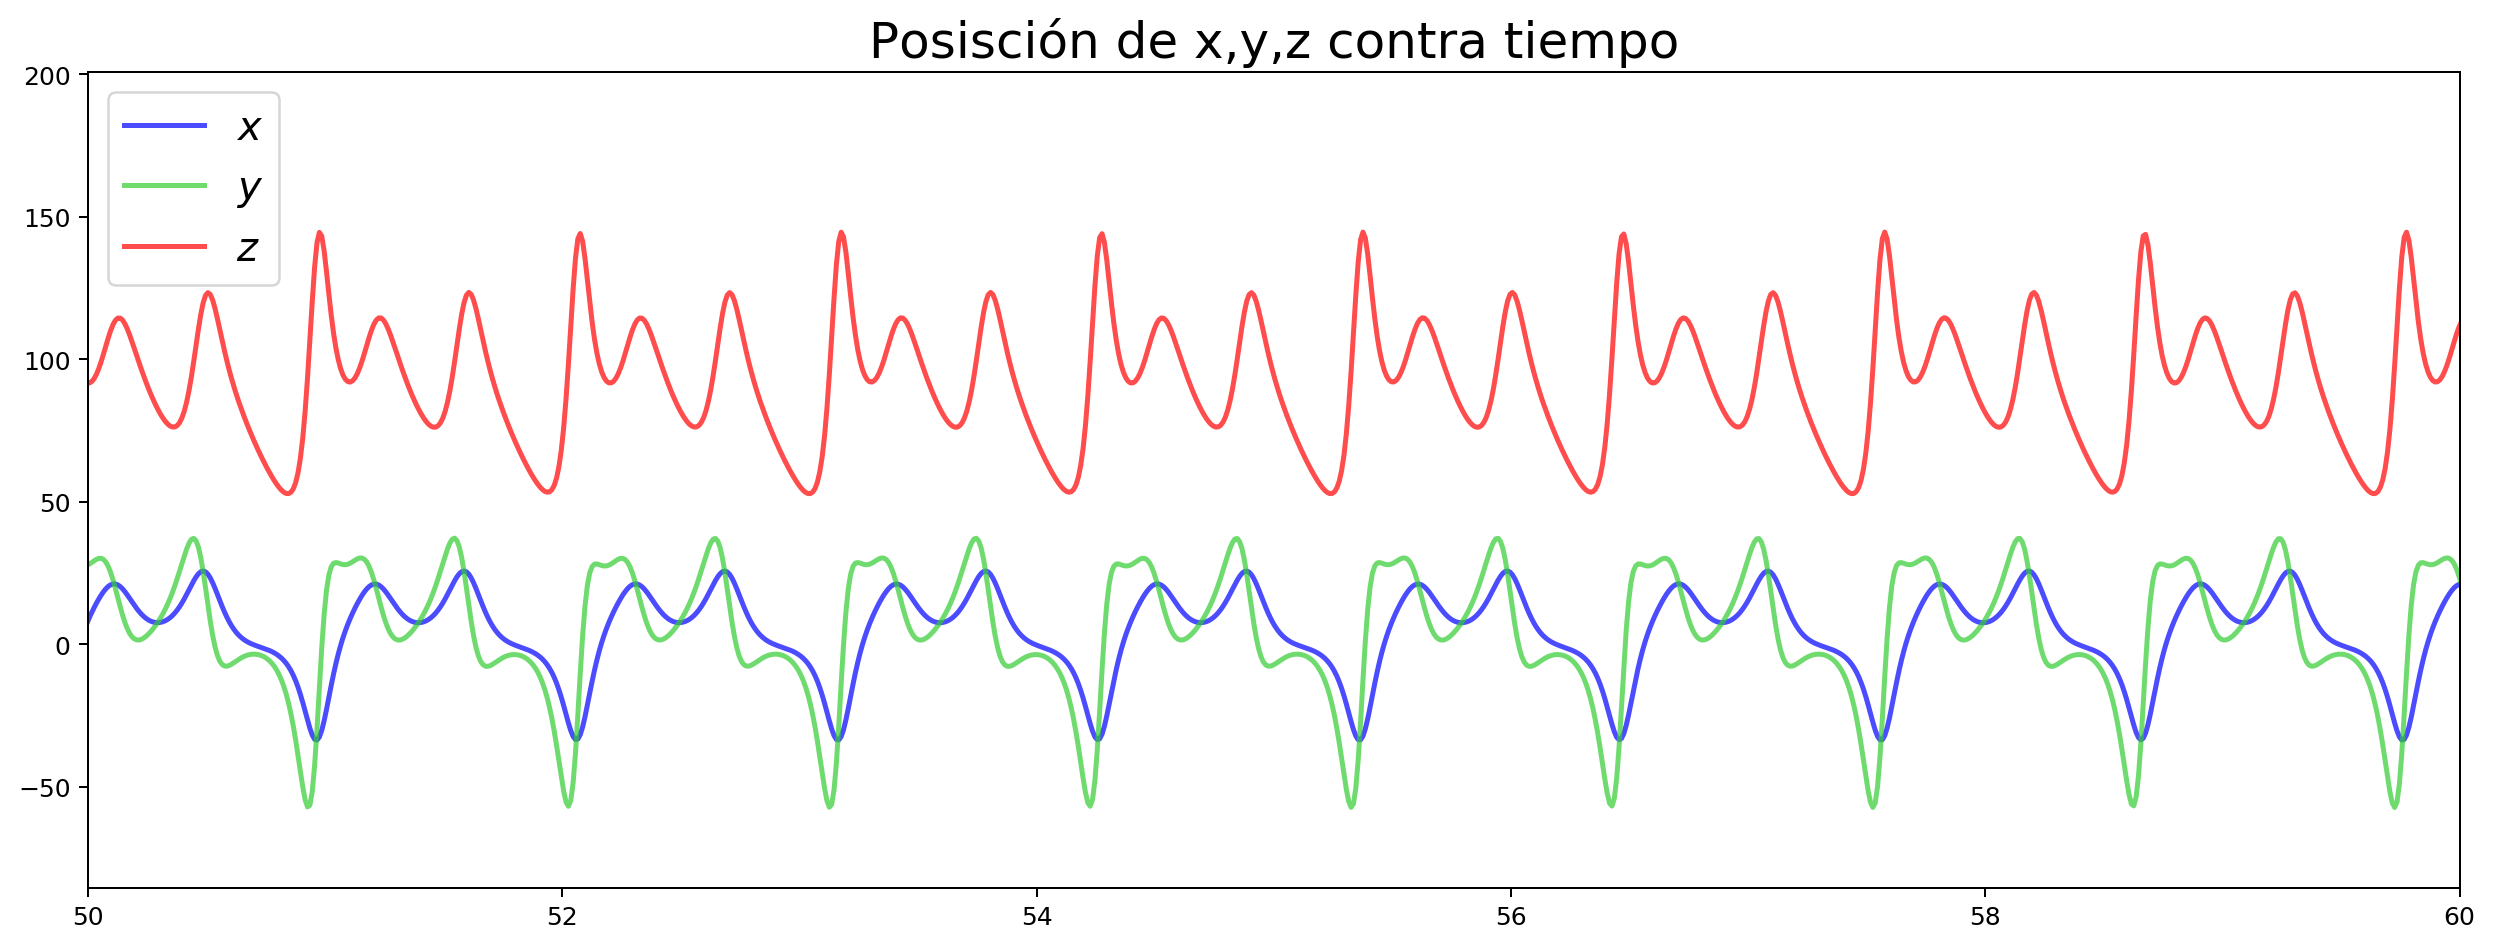
\includegraphics[width=1\textwidth]{PosicionZoom.png}
\end{center}

Los siguientes ejemplos se realizaron de la misma manera, analizándose los efectos que el cambio de las constantes puede traer al sistema.

\subsection{Ejemplo 2}
Valores: $\sigma = 28, \beta = 4 \textup{ y } \rho = 46.92$:

En la primera gráfica puede observar como el atractor es más grueso a comparación del ejemplo 1, sin embargo, estos dos gráficas parecen girar al rededor de los mismos puntos.
\begin{center}
    \includegraphics[width=1\textwidth]{lorenz-attractor-3d_2.png}
\end{center}
Las siguientes gráficas se observan más densas, haciendo más notorias las figuras del ejemplo anterior, solo que ahora los orificios de los puntos orbitados son más pequeños.

\begin{center}
    \includegraphics[width=1\textwidth]{lorenz-attractor-phase-_2.png}
\end{center}

Las gráficas de posición contra tiempo, muestran como el movimiento fue más caótico debido a que cambiaban de orbita en menor tiempo.
\begin{center}
    \includegraphics[width=1\textwidth]{Posicion_2.png}
    \includegraphics[width=1\textwidth]{PosicionZoom_2.png}
\end{center}

\subsection{Ejemplo 3}
Valores: $\sigma = 10, \beta = 8/3 \textup{ y } \rho = 99.96$:

\begin{center}
    \includegraphics[width=.9\textwidth]{lorenz-attractor-3d_3.png}
\end{center}
A pesar de que solo cambia el valor de la constante $\rho$, el movimiento del atractor sufre grandes cambios, pierde simetría y toma distintos valores a los que se habían tomado anteriormente. Esto se puede notar tanto en la grádica de 3 dimensiones como en las de la fase, donde en estas ultimas, muestra las figuras de los ejemplos anteriores pero deformadas, sobre todo en los valores positivos de las variables.
\begin{center}
    \includegraphics[width=1\textwidth]{lorenz-attractor-phase-_3.png}
\end{center}
Por último, en las gráficas de posición contra tiempo se puede observar una periodiocidad en sus movimientos, además las variables x y y toman mayormente valores negativos.
\begin{center}
    \includegraphics[width=1\textwidth]{Posicion_3.png}
    \includegraphics[width=1\textwidth]{PosicionZoom_3.png}
\end{center}

\section{Conclusión}
Me parece que analizar los fénomenos caóticos con herramientas como las que se utilizaron para resolver este sistema, representa una sencilla forma de abordarlos, ya que ver las gráficas y sus proyecciones ayuda a que te des una idea de como funciona el sistema y sus características.

\section{Bibliografía}
Lorenz system. (2018). En.wikipedia.org. Recuperado el 26 de Abril de 2018, de \url{https://en.wikipedia.org/wiki/Lorenz_system}
\end{document}
